\documentclass[a4paper]{article}
\usepackage{amsfonts}
\usepackage{amsmath}
\usepackage{amssymb}
\usepackage{graphicx}  
\usepackage{cancel}

\newcommand{\degree}{^{\circ}}
\newcommand{\cis}{\operatorname{cis}}
\newcommand{\Bgsin}{\operatorname{Bgsin}}
\newcommand{\Bgcos}{\operatorname{Bgcos}}
\newcommand{\Bgtan}{\operatorname{Bgtan}}
\newcommand{\limit}{\lim\limits}
\newcommand{\summation}{\displaystyle\sum}
\newcommand{\dom}{\operatorname{dom}}
\newcommand{\Int}{\displaystyle\int}

\begin{document}
  
\noindent \large Auteur: Rune Suy \\
\noindent \large Studierichting: Informatica\\
\noindent \large Oefeningenreeks 5G nr. 2.1\\

\medskip

\normalsize

$f(x) = -x^2 + 4x$\\

$-x^2 + 4x = 0 \Leftrightarrow x(4-x)=0 \Leftrightarrow x=0$ of $x=4$\\

$V = \pi \Int_0^4 (-x^2 +4x)^2 dx$\\

$= \pi \Int_0^4 (x^4 - 8x^3 + 16x^2) dx$\\

$ = \pi \left[ \Int_0^4 x^4 dx - 8\Int_0^4 x^3 dx + 16 \Int_0^4x^2dx  \right]$\\

$= \pi \left[ \left[ \dfrac{x^5}{5} \right]_0^4 - 8 \left[ \dfrac{x^4}{4} \right]_0^4 + 16 \left[ \dfrac{x^3}{3} \right]_0^4  \right]$\\

$= \pi \left(\dfrac{3072}{15} - \dfrac{7680}{15} + \dfrac{5120}{15}\right)$\\

$= \dfrac{512\pi}{15}$\\
\newpage

\begin{figure}[h]
    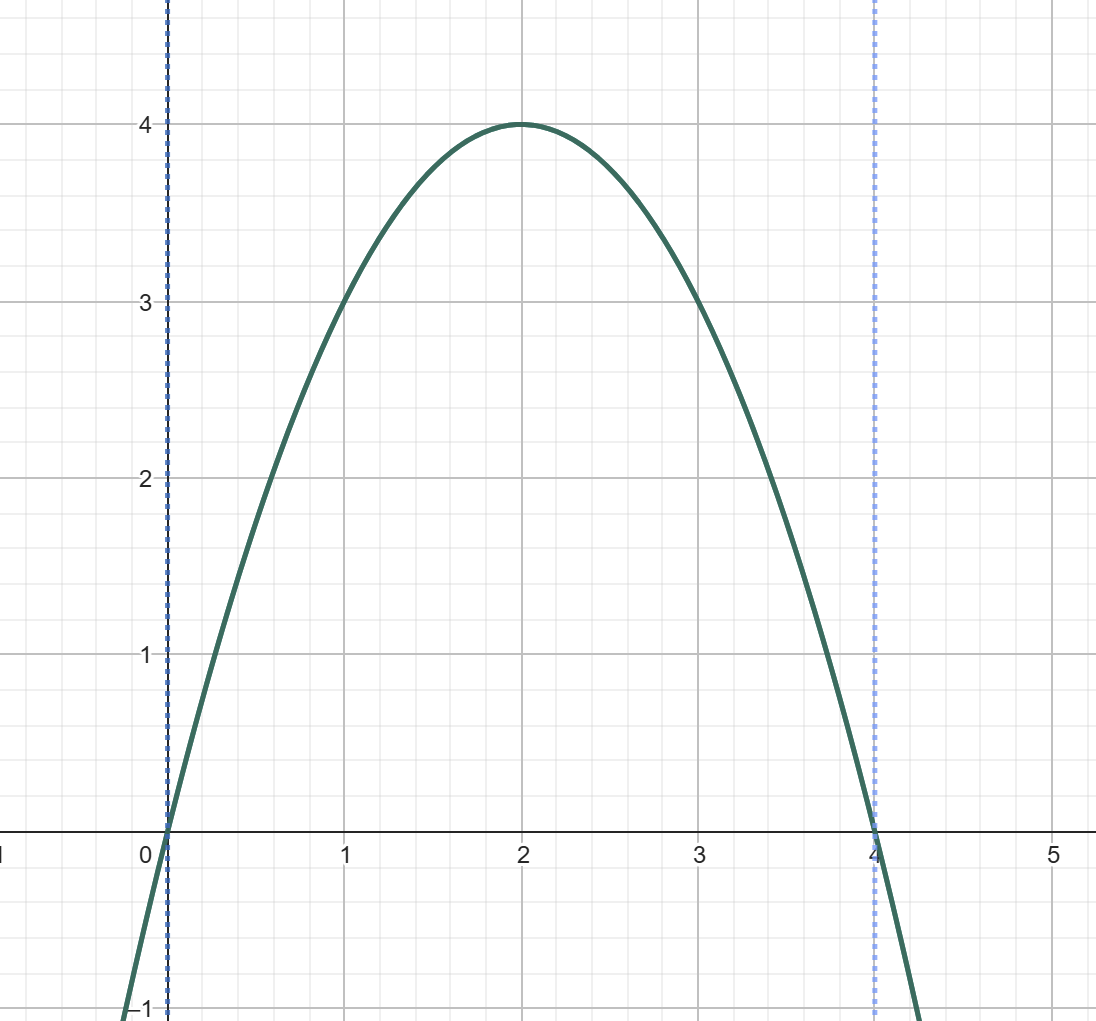
\includegraphics[width=\linewidth]{5G-2.1-rune.suy.INF.png}\\
\end{figure}

\begin{thebibliography}{999}
%\bibitem{a} Referentie
\end{thebibliography}
\end{document} 
